\documentclass[11pt]{elegantbook}
\definecolor{structurecolor}{RGB}{40,58,129}
\linespread{1.6}
\setlength{\footskip}{20pt}
\setlength{\parindent}{0pt}
\newcommand{\argmax}{\operatornamewithlimits{argmax}}
\newcommand{\argmin}{\operatornamewithlimits{argmin}}
\elegantnewtheorem{proof}{Proof}{}{Proof}
\elegantnewtheorem{claim}{Claim}{prostyle}{Claim}
\DeclareMathOperator{\col}{col}
\title{\textbf{Economic Theory and Some Useful Math}}
\author{Wenxiao Yang}
\institute{Haas School of Business, University of California Berkeley}
\date{2023}
\setcounter{tocdepth}{2}
\cover{cover.png}
\extrainfo{All models are wrong, but some are useful.}

% modify the color in the middle of titlepage
\definecolor{customcolor}{RGB}{9,119,119}
\colorlet{coverlinecolor}{customcolor}
\usepackage{cprotect}

\addbibresource[location=local]{reference.bib} % bib

\begin{document}

\maketitle
\frontmatter
\tableofcontents
\mainmatter


\chapter{Market Design}
Based on
\begin{enumerate}[$\circ$]
    \item UC Berkeley MATH 272 23Fall, Alexander Teytelboym
    \item  Jehle, G., Reny, P.: Advanced Microeconomic Theory . Pearson, 3rd ed. (2011). Ch. 6.
    \item Notes on Social Choice and Welfare, Alejandro Saporiti
\end{enumerate}
\section{Individual Choice to Preferences}
\begin{definition}[Unitility Function]
    \normalfont
    We can say a function $u: X \rightarrow \mathbb{R}$ represents $\succeq$ if $\forall x,y\in X$, $$x\succeq y \Leftrightarrow u(x)\geq u(y)$$
\end{definition}

\begin{proposition}
    If $\exists$ a function $u: X \rightarrow \mathbb{R}$ represents $\succeq$, then $\succeq$ is rational (i.e., completeness and transitivity)
\end{proposition}
\begin{note}
    The reverse may not true.
\end{note}

Let $\mathcal{B}=2^X$ (all subsets of $X$) and $B\in \mathcal{B}$ be the all potential alternatives that can be chosen.

The choice of an agent can be represented by $C(B)\subseteq B, \forall B\in \mathcal{B}$.


\subsection{Weak Axiom of Revealed Preference (WARP)}
\begin{definition}[Weak Axiom of Revealed Preference]
    \normalfont
    Given a choice structure $(C,\mathcal{B})$ satisfies \textbf{WARP}. If $\exists B\in \mathcal{B}$ with $x,y\in B$, such that $x\in C(B)$. Then, $\forall B'\in \mathcal{B}$ with $x,y\in B'$, $y\in C(B') \Rightarrow x\in C(B')$.
\end{definition}

\begin{proposition}[Rational $\Rightarrow$ WARP]
    Given $\succeq$ is rational, then $(C^*_{\succeq},\mathcal{B})$ satisfies WARP.\\
    ($C^*_{\succeq}$ is the choice rule that picks the maximal alternatives by $\succeq$)
\end{proposition}


\section{Social Choice}
Notations:
\begin{enumerate}
    \item We consider \underline{finite} set of alternatives $X$ and \underline{finite} set of agents $I$.
    \item We use $\mathcal{B}$ to denotes the set of all preference relations.
    \item We use $\mathcal{R}\subseteq \mathcal{B}$ to denotes the set of all rational preference relations.
    \item We use $\succeq\in \mathcal{R}$ to represents individual rational preference relation.
\end{enumerate}

\subsection{Social Welfare Function and Properties}
\begin{definition}[Social Welfare Function (SWF)]
    \normalfont
    A \textbf{social welfare function} (SWF) is a mapping $$f: \mathcal{A}\subseteq \mathcal{R}^I\rightarrow \mathcal{B}$$
    $\trianglerighteq=f(\succeq_1,...,\succeq_I)$ is interpreted as the \textbf{social preference relation}. It doesn't need to be rational (i.e., complete and transitive).
\end{definition}

\begin{definition}[SWF's Properties]
    \normalfont
    A social welfare function $f: \mathcal{A}\rightarrow \mathcal{B}$
    \begin{enumerate}[$\circ$]
        \item has \textbf{unrestricted domain} (UD) if $\mathcal{A}=\mathcal{R}^n$;
        \item is \textbf{transitive} (T) if $f(\succeq_1,...,\succeq_I)$ is transitive for all $(\succeq_1,...,\succeq_I)\in \mathcal{A}$;
        \item is \textbf{nondictatorial} (ND) if there is no agent $i\in I$ such that $\forall \{x,y\}\subseteq X$ $x\succeq_i y \Rightarrow x\trianglerighteq y$.
        \item is \textbf{weakly Paretian} (PA) if, $\forall \{x,y\}\subseteq X$ and any preference profile $(\succeq_1,...,\succeq_I)\in \mathcal{A}$, we have $x\succeq_i y,\forall i\in I \Rightarrow x\trianglerighteq y$.
        \item is \textbf{independent of irrelevant alternatives} (IIA) if, $\forall \{x,y\}\subseteq X$, and any $\succeq$ and $\succeq'$ with $\succeq_i\mid_{x,y}=\succeq'_i\mid_{x,y}, \forall i\in I$, if $x\trianglerighteq y$ then $x\trianglerighteq' y$.
    \end{enumerate}
\end{definition}


\subsection{Arrow's Theorem}
\begin{theorem}[Arrow's impossibility theorem]
    Suppose $|X|\geq 3$, $\mathcal{A}=\mathcal{R}^I$ (UD). Then if a SWF $f$ satisfies T, PA, and IIA, then it fails to be ND.
\end{theorem}















\chapter{Signalling Game}
Based on
\begin{enumerate}[$\circ$]
    \item "Kreps, D. M., \& Sobel, J. (1994). Signalling. \textit{Handbook of game theory with economic applications}, 2, 849-867."
    \item 
\end{enumerate}

\section{Canonical Game}
\begin{definition}[Canonical Game]
    \normalfont
    \begin{enumerate}
        \item There are two players: $\mathbf{S}$ (sender) and $\mathbf{R}$ (receiver).
        \item $\mathbf{S}$ holds more information than $\mathbf{R}$: the value of some random variable $t$ with support $\mathcal{T}$. (We say that $t$ is the \textbf{type} of $\mathbf{S}$)
        \item Prior belief of $\mathbf{R}$ concerning $t$ are given by a probability distribution $\rho$ over $\mathcal{T}$ (common knowledge)
        \item $\mathbf{S}$ sends a \textbf{signal $s\in \mathcal{S}$} to $\mathbf{R}$ drawn from a signal set $\mathcal{S}$.
        \item $\mathbf{R}$ receives this signal, and then takes an \textbf{action} $a\in \mathcal{A}$ drawn from a set $\mathcal{A}$ (which could depend on the signal $s$ that is sent).
        \item $\mathbf{S}$'s payoff is given by a function $u: \mathcal{T}\times \mathcal{S} \times \mathcal{A} \rightarrow \mathbb{R}$ and $\mathbf{R}$'s payoff is given by a function $v: \mathcal{T}\times \mathcal{S} \times \mathcal{A} \rightarrow \mathbb{R}$.
    \end{enumerate}
\end{definition}

\section{Nash Equilibrium}
\begin{definition}[Strategy]
    \normalfont
    A \textbf{behavior strategy} for $\mathbf{S}$ is given by a function $\sigma: \mathcal{T}\times\mathcal{S} \rightarrow [0,1]$ such that $\sum_s \sigma(t,s)$ for each $t$.\\
    A \textbf{behavior strategy} for $\mathbf{R}$ is given by a function $\alpha: \mathcal{S}\times\mathcal{A} \rightarrow [0,1]$ such that $\sum_a \alpha(s,a)$ for each $t$.
\end{definition}

\begin{definition}[Nash Equilibrium]
    \normalfont
    Behavior strategies $\alpha$ and $\sigma$ form a \textbf{Nash equilibrium} if and only if
    \begin{enumerate}
        \item For all $t\in \mathcal{T}$,
        \begin{center}
            $\sigma(t,s)>0$ implies $\sum_a \alpha(s,a)u(t,s,a) = \max_{s'\in \mathcal{S}}\left(\sum_a \alpha(s',a)u(t,s',a)\right)$
        \end{center}
        \item For each $s\in \mathcal{S}$ such that $\sum_{t}\sigma(t,s)\rho(t)>0$,
        \begin{center}
            $\alpha(s,a)>0$ implies $\sum_{t}\mu(t;s)v(t,s,a) = \max_{a'}\sum_{t}\mu(t;s)v(t,s,a')$
        \end{center}
        where $\mu(t;s)$ is the $\mathbb{R}$'s posterior belief about $t$ given $s$, $\mu(t;s)=\frac{\sigma(t,s)\rho(t)}{\sum_{t'}\sigma(t',s)\rho(t')}$ if $\sum_t\sigma(t,s)\rho(t)>0$ and $\mu(t;s)=0$ otherwise.
    \end{enumerate}
\end{definition}

\begin{definition}[Separating \& Pooling Equilibrium]
    \normalfont
    An equilibrium $(\sigma,\alpha)$ is called a \textbf{separating} equilibrium if each type $t$ sends different signals; i.e., the set $\mathcal{S}$ can be partitioned into (disjoint) sets $\{\mathcal{S}_t; t\in \mathcal{S}\}$ such that $\sigma(t, \mathcal{S}_t) = 1$. An equilibrium $(\sigma,\alpha)$ is called a \textbf{pooling} equilibrium if there is a single signal $s^*$ that is sent by all types; i.e., $\sigma(t, s^*) = 1$ for all $t\in \mathcal{T}$.
\end{definition}


\section{Single-crossing}

\subsection{Situation over real line}
Consider the situation that $\mathcal{T},\mathcal{S},\mathcal{A}\subseteq \mathbb{R}$ and $\geq$ is the usual "greater than or equal to" relationship.

\begin{enumerate}
    \item We let $\Delta \mathcal{A}$ denote the set of probability distributions on $\mathcal{A}$.
    \item For each $s\in \mathcal{S}$ and $\mathcal{T}'\subseteq \mathcal{T}$, we let $\Delta\mathcal{A}(s,T')$ be the set of mixed strategies that are the best responses by $\mathbf{R}$ to $s\in \mathcal{S}$ for some probability distribution with support $\mathcal{T}'$.
    \item For $\alpha\in \Delta\mathcal{A}$, we write $u(t,s,\alpha)\triangleq \sum_{a\in \mathcal{A}}u(t,s,a)\alpha(a)$.
\end{enumerate}

\begin{definition}[Single-crossing]
    \normalfont
    The data of the game are said to satisfy the \textbf{single-crossing property} if the following holds: If $t\in \mathcal{T}$, $(s,\alpha)\in \mathcal{S}\times \Delta\mathcal{A}$ and $(s',\alpha')\in \mathcal{S}\times \Delta\mathcal{A}$ are such that $\alpha\in \Delta\mathcal{A}(s,\mathcal{T})$, $\alpha'\in \Delta\mathcal{A}(s',\mathcal{T})$, $s>s'$ and $u(t,s,\alpha)\geq u(t,s',\alpha')$, then for all $t'\in T$ such that $t'>t$, $u(t',s,\alpha)\geq u(t',s',\alpha')$.
\end{definition}




\chapter{Tools for Comparative Statics}
Consider the function $f:(0,2\pi) \times \mathbb{R} \rightarrow \mathbb{R}$ s.t. $$f(x,a)=\sin x+a$$
Let $X=(0,2\pi)$ and let $f_a(x) = f(x, a) = \sin x + a$ denote the perturbed function for fixed $a$.



\section{Regular and Critical Points and Values}
\subsection{Rank of Derivatives $\textnormal{Rank} df_x=\textnormal{Rank} Df(x)$}
Suppose $X \subseteq \mathbb{R}^n$ is open. Suppose $f : X \rightarrow \mathbb{R}^m$ is differentiable at $x \in X$, and let $W = \{e_1, . . . , e_n\}$ denote the standard basis of $\mathbb{R}^n$. Then $df_x \in L(\mathbb{R}^n, \mathbb{R}^m)$, and
\begin{equation}
    \begin{aligned}
        \textnormal{Rank} df_x &= \dim \textnormal{Im}(df_x)\\
        &= \dim \textnormal{span}\{df_x(e_1), . . . , df_x(e_n)\}\\
        &= \dim \textnormal{span}\{Df(x)e_1, . . . , Df(x)e_n\}\\
        &= \dim \textnormal{span}\{\textnormal{column 1 of }Df(x), . . . , \textnormal{column n of }Df(x)\}\\
        &=\textnormal{Rank} Df(x)
    \end{aligned}
    \nonumber
\end{equation}
Thus,
$$\textnormal{Rank} df_x\leq\min\{m,n\}$$
$df_x$ has \textbf{full rank} if $\textnormal{Rank} df_x=\min\{m,n\}$, that is, is $df_x$ has the maximum possible rank.

\subsection{Regular and Critical Points and Values}
\begin{definition}[Regular and Critical Points and Values]
    \normalfont
    Suppose $X \subseteq \mathbb{R}^n$ is open. Suppose $f : X \rightarrow \mathbb{R}^m$ is differentiable at $x \in X$.
    \begin{enumerate}
        \item $x$ is a \textbf{regular point} of $f$ if $\textnormal{Rank} df_x=\min\{m,n\}$.
        \item $x$ is a \textbf{critical point} of $f$ if $\textnormal{Rank} df_x<\min\{m,n\}$.
        \item $y$ is a \textbf{critical value} of $f$ if  there exists $x \in f^{-1}(y)$ such that $x$ is a critical point of $f$.
        \item $y$ is a \textbf{regular value} of $f$ if $y$ is not a critical value of $f$.
    \end{enumerate}
\end{definition}
\begin{note}
    Notice that if $y \notin f(X)$, so $f^{-1}(y) = \emptyset$, then $y$ is automatically a regular value of $f$.
\end{note}

\begin{example}
    Suppose $f(x,y)=(\sin x,\cos y)$, $Df(x,y)=\begin{bmatrix}
        \cos x&	0\\
        0&	-\sin y
    \end{bmatrix}$. Critical point: $\{(\frac{k\pi}{2}, \mathbb{R}): k\in 2\mathbb{Z}+1\}\cup\{(\mathbb{R},k\pi): k\in \mathbb{Z}\}$; Critical values: $\{(x,y): x=1\textnormal{ or }x=-1 \textnormal{ or }y=1\textnormal{ or }y=-1\}$
\end{example}


\section{Inverse and Implicit Function Theorem}
\subsection{Inverse Function Theorem}
Using Taylor's theorem to approximate
\begin{equation}
    \begin{aligned}
        f(x)=f(x_0)+Df(x_0)(x-x_0)+o(x-x_0)
    \end{aligned}
    \nonumber
\end{equation}
The requirement of "regular point" is necessary for the $Df(x_0)$ being invertible.
\begin{theorem}[Inverse Function Theorem]
    Suppose $X \subseteq \mathbb{R}^n$ is open. Suppose $f : X \rightarrow \mathbb{R}^n$ is $C^1$ on $X$, and $x_0\in X$. If $\det Df(x_0)\neq 0$ (i.e., $x_0$ is a regular point of $f$), then there are open neighborhoods $U$ of $x_0$ and $V$ of $f(x_0)$ s.t.
    \begin{equation}
        \begin{aligned}
            &f:U \rightarrow V \textnormal{ is bijective (on-to-on and onto)}\\
            &\exists\ f^{-1}:V \rightarrow U \textnormal{ is }C^1\\
            &Df^{-1}(f(x_0))=[Df(x_0)]^{-1}\\
            &\textnormal{(In $\mathbb{R}$, $(f^{-1})'(f(x_0))=(f'(x_0))^{-1}$)}
        \end{aligned}
        \nonumber
    \end{equation}
    If in addition $f \in C^k$, then $f^{-1} \in C^k$.
\end{theorem}

\subsection{Implicit Function Theorem}
Using Taylor's theorem to approximate
\begin{equation}
    \begin{aligned}
        f(x,a)=f(x_0,a_0)+Df(x_0,a_0)(x-x_0)+Df(x_0,a_0)(a-a_0)+\textnormal{remainder}
    \end{aligned}
    \nonumber
\end{equation}
The requirement of "regular point" is necessary for the $Df(x_0,a_0)$ being invertible.

We want to know how the function $x^*(a)$ changes with keeping $f(x^*,a)=0$.
\begin{theorem}[Implicit Function Theorem]
    Suppose $X \subseteq \mathbb{R}^n$ and $A \subseteq \mathbb{R}^p$ are open and $f : X \times A \rightarrow \mathbb{R}^n$ is $C^1$. Suppose $f(x_0, a_0) = 0$ and $\det(D_x f(x_0, a_0)) \neq 0$, i.e. $x_0$ is a regular point of $f(\cdot, a_0)$. Then there are open neighborhoods $U$ of $x_0$ ($U \subseteq X$) and $W$ of $a_0$ such that
    $$\forall a\in W,\ \exists ! x\in U \textnormal{ s.t. }f(x,a)=0$$
    For each $a \in W$ let $g(a)$ be that unique $x$. Then $g : W \rightarrow U$ is $C^1$ and $$Dg(a_0)=-[D_x f(x_0, a_0)]^{-1}[D_a f(x_0, a_0)]$$
    If in addition $f \in C^k$, then $g \in C^k$.
\end{theorem}
\subsection{Prove Implicit Function Theorem Given Inverse Function Theorem}
\begin{proof}
    \begin{enumerate}
        \item Firstly, we prove "$g$ is differentiable":
        The "change of $a$" incurs the value change:
        \begin{equation}
            \begin{aligned}
                f(x_0,a_0+h)&=f(x_0,a_0)+D_af(x_0,a_0)h+o(h)\\
                &=D_af(x_0,a_0)h+o(h)\\
            \end{aligned}
            \nonumber
        \end{equation}
        Find a $\Delta x$ such that the new $x$ can let the value go back to $0$, i.e., $f(x_0+\Delta x,a_0+h)=0$. That is,
        \begin{equation}
            \begin{aligned}
                g(a_0+h)=x_0+\Delta x
            \end{aligned}
            \nonumber
        \end{equation}
        To prove "$g$ is differentiable", we want to prove "$\exists T\in L(A,X)$ s.t. $\Delta x=T(h)+o(h)$"
        \begin{equation}
            \begin{aligned}
                0&=f(x_0+\Delta x,a_0+h)\\
                &=f(x_0,a_0)+D_xf(x_0,a_0+h)\Delta x+ D_a f(x_0,a_0)h+o(\Delta x)+o(h)\\
                &=D_xf(x_0,a_0+h)\Delta x+ D_a f(x_0,a_0)h+o(\Delta x)+o(h)\\
                D_x f(x_0,a_0+h)\Delta x&=-D_a f(x_0,a_0)h+o(\Delta x)+o(h)
            \end{aligned}
            \nonumber
        \end{equation}
        Because $f$ is $C^1$ and the determinant is a continuous function of the entries of the matrix, $\det D_xf(x_0, a_0 + h) \neq 0$ for $h$ sufficiently small, so
        \begin{equation}
            \begin{aligned}
                \Delta x&= -[D_x f(x_0,a_0+h)]^{-1}D_a f(x_0,a_0)h+o(\Delta x)+o(h)\\
                \textnormal{Since $f\in C^1$, }\Delta x&= -[D_x f(x_0,a_0)+o(1)]^{-1}D_a f(x_0,a_0)h+o(\Delta x)+o(h)\\
                \textnormal{Since $f\in C^1$, }\Delta x&= -[D_x f(x_0,a_0)]^{-1}D_a f(x_0,a_0)h+o(\Delta x)+o(h)
            \end{aligned}
            \nonumber
        \end{equation}
        Hence, "$g$ is differentiable" is proved and the derivative of $g$ is $Dg(a_0)=-[D_x f(x_0,a_0)]^{-1}[D_a f(x_0,a_0)]$.
        \item Secondly, given the "$g$ is differentiable", we can also compute the derivative by
        \begin{equation}
            \begin{aligned}
                Df(g(a),a)(a_0)&=0\\
                D_xf(x_0,a_0)Dg(a_0)+D_af(x_0,a_0)&=0\\
                Dg(a_0)&=-[D_x f(x_0,a_0)]^{-1}D_a f(x_0,a_0)
            \end{aligned}
            \nonumber
        \end{equation}
    \end{enumerate}
\end{proof}







\begin{example}
    $f: \mathbb{R}^3 \rightarrow \mathbb{R}^2$, $f((3,-1,2))=(0,0)$, $Df(3,-1,2)=\begin{bmatrix}
        1&2&1\\
        1&-1&1
    \end{bmatrix}$. Then,
    let $(x_0,a_0)=(3,-1,2)$, where $x_0=3$ and $a_0=(-1,2)$. Or, we can let $(x_0,a_0)=(3,-1,2)$, where $x_0=(3,-1)$ and $a_0=2$.
\end{example}

\subsection{Prove Inverse Function Theorem Given Implicit Function Theorem}
\begin{proof}[Prove Inverse Function Theorem Given Implicit Function Theorem]
    Define $F:X\times \mathbb{R}^n$ s.t. $F(x,y)=y-f(x)$. Let $y_0=f(x_0)$.
    \begin{equation}
        \begin{aligned}
            D_x F(x,y)=-Df(x),\ D_y F(x,y)=I_{n\times n}
        \end{aligned}
        \nonumber
    \end{equation}
    According to the implicit function theorem, there are open sets $U \subseteq X$ and $V \subseteq \mathbb{R}^n$ such that $x_0 \in U$, $y_0 \in V$ and a function $g : V \rightarrow U$ differentiable at $y_0$ such that $F(g(y), y) = 0$ for all $y \in V$. So, $0=F(g(y),y)=y-f(g(y))$, we have $f(g(y))=y$, that is $g=f^{-1}$.
    $f: U \rightarrow V$ is bijective because it has inverse $g : V \rightarrow U$.

    By the implicit function theorem, $g(y)$ is differentiable and
    \begin{equation}
        \begin{aligned}
            Df^{-1}(y_0)=Dg(y_0)=-[D_x F(x_0,y_0)]^{-1}[D_y F(x_0,y_0)]=[Df(x_0)]^{-1}
        \end{aligned}
        \nonumber
    \end{equation}
    where $y_0=f(x_0)$.
    
    By the implicit function theorem, the $g=f^{-1}$ is $C^k$ if $f$ is $C^k$.

    All in all, the inverse function theorem is proved.
\end{proof}

\subsection{Example: Using Implicit Function Theorem in Comparative Statics}
\begin{example}
    Let us consider a firm that produces a good $y$; it uses two inputs $x_1$ and $x_2$. The firm sells the output and acquires the inputs in competitive markets: The market price of $y$ is $p$, and the cost of each unit of $x_1$ and $x_2$ are $w_1$ and $w_2$ respectively. Its technology is given by $f : \mathbb{R}^2_+ \rightarrow \mathbb{R}_+$, where $f (x_1, x_2) = x_1^ax_2^b$, $a + b < 1$. Its profits take the form
    \begin{equation}
        \begin{aligned}
            \pi(x_1,x_2; p, w_1,w_2)=p x_1^ax_2^b-w_1x_1-w_2x_2
        \end{aligned}
        \nonumber
    \end{equation}
    The firm selects $x_1$ and $x_2$ in order to maximize profits. \textbf{We aim to know how its choice of $x_1$ and $x_2$ is affected by a change in $w_1$}.

    Assuming an interior solution, the first-order conditions of this optimization problem are
    \begin{equation}
        \begin{aligned}
            \frac{\partial \pi}{\partial x_1}(x_1^*,x_2^*;p,w_1,w_2)=pa(x_1^*)^{a-1}(x_2^*)^b-w_1=0\\
            \frac{\partial \pi}{\partial x_2}(x_1^*,x_2^*;p,w_1,w_2)=pb(x_1^*)^{a}(x_2^*)^{b-1}-w_2=0
        \end{aligned}
        \nonumber
    \end{equation}
    for some $(x_1, x_2) = (x_1^*,x_2^*)$.

    Let us define
    \begin{equation}
        \begin{aligned}
            F(x_1^*,x_2^*;p,w_1,w_2)=
            \begin{bmatrix}
                pa(x_1^*)^{a-1}(x_2^*)^b-w_1\\
                pb(x_1^*)^{a}(x_2^*)^{b-1}-w_1
            \end{bmatrix}
        \end{aligned}
        \nonumber
    \end{equation}
    Jacobian matrices are
    \begin{equation}
        \begin{aligned}
            D_{(x_1,x_2)}F(x_1^*,x_2^*;p,w_1,w_2)=\begin{bmatrix}
                pa(a-1)(x_1^*)^{a-2}(x_2^*)^b&pab(x_1^*)^{a-1}(x_2^*)^{b-1}\\
                pab(x_1^*)^{a-1}(x_2^*)^{b-1}&pb(b-1)(x_1^*)^{a}(x_2^*)^{b-2}
            \end{bmatrix}
        \end{aligned}
        \nonumber
    \end{equation}
    \begin{equation}
        \begin{aligned}
            D_{w_1}F(x_1^*,x_2^*;p,w_1,w_2)
            &=
            \begin{bmatrix}
                -1\\
                0
            \end{bmatrix}
        \end{aligned}
        \nonumber
    \end{equation}
    By the implicit function theorem, we can get
    \begin{equation}
        \begin{aligned}
            \begin{bmatrix}
                \frac{\partial x_1^*}{\partial w_1}\\
                \frac{\partial x_2^*}{\partial w_1}
            \end{bmatrix}&=-[D_{(x_1,x_2)}F(x_1^*,x_2^*;p,w_1,w_2)]^{-1}[D_{w_1}F(x_1^*,x_2^*;p,w_1,w_2)]\\
            &=[D_{(x_1,x_2)}F(x_1^*,x_2^*;p,w_1,w_2)]^{-1}\begin{bmatrix}
                1\\
                0
            \end{bmatrix}
        \end{aligned}
        \nonumber
    \end{equation}
\end{example}

\subsection{Corollary: $a \rightarrow \{x\in X: f(x,a)=0\}$ is lhc}
\begin{corollary}
    Suppose $X \subseteq \mathbb{R}^n$ and $A \subseteq \mathbb{R}^p$ are open and $f : X \times A \rightarrow \mathbb{R}^n$ is $C^1$. If $0$ is a regular value of $f(\cdot, a_0)$, then the correspondence $$a \rightarrow \{x\in X: f(x,a)=0\}$$
    is \textbf{lower hemicontinuous} at $a_0$.
\end{corollary}


\section{Transversality and Genericity}
\subsection{Lebesgue Measure Zero}
\begin{definition}[Lebesgue Measure Zero]
    \normalfont
    Suppose $A \subseteq \mathbb{R}^n$. $A$ has \textbf{Lebesgue measure zero} if for every $\varepsilon > 0$ there is a countable collection of rectangles $I_1, I_2, . . .$ such that
    \begin{equation}
        \begin{aligned}
            \sum_{k=1}^\infty\textnormal{Vol}(I_k)<\varepsilon \textnormal{ and }A\subseteq \cup_{k=1}^\infty I_k
        \end{aligned}
        \nonumber
    \end{equation}
    Here by a rectangle we mean $I_k = \times^n_{j=1}(a^k_j , b^k_j)=\{x\in \mathbb{R}^n: x_j\in (a^k_j , b^k_j), \forall j\}$ for some $a^k_j < b^k_j \in \mathbb{R}$, and
    \begin{equation}
        \begin{aligned}
            \textnormal{Vol}(I_k)=\prod_{j=1}^n|b^k_j-a^k_j|
        \end{aligned}
        \nonumber
    \end{equation}
\end{definition}

\begin{example}
    \begin{enumerate}
        \item “Lower-dimensional” sets have Lebesgue measure zero. For example, $A=\{x\in\mathbb{R}^2:x_2=0\}$
        \item Any \textbf{finite} set has Lebesgue measure zero in $\mathbb{R}^n$.
        \item \textbf{Finite Union} of sets that have Lebesgue measure zero has Lebesgue measure zero: If $A_n$ has Lebesgue measure zero $\forall n$ then $\cup_{n\in N}A_n$ has Lebesgue measure zero.
        \item Every \textbf{countable} set (e.g. $\mathbb{Q}$) has Lebesgue measure zero.
        \item No open set in $\mathbb{R}^n$ has Lebesgue measure zero.
    \end{enumerate}
\end{example}


\subsection{Sard's Theorem}
\begin{theorem}[Sard's Theorem]
    Let $X \subseteq \mathbb{R}^n$ be open, and $f : X \rightarrow \mathbb{R}^m$ be $C^r$ with $r \geq 1 + max\{0, n - m\}$. Then the set of all critical values of $f$ has Lebesgue measure zero.
\end{theorem}

\subsection{Transversality Theorem}
\begin{theorem}[Transversality Theorem]
    Let $X \subseteq \mathbb{R}^n$ and $A \subseteq \mathbb{R}^p$ be open, and $f : X \times A \rightarrow \mathbb{R}^m$ be $C^r$ with $r \geq 1 + max\{0, n - m\}$. Suppose that $0$ is a regular value of $f$ (that is all $(x,a)$ such that $f(x,a)=0$ are regular points). Then,
    \begin{enumerate}
        \item $\exists A_0 \subseteq A$ such that $A \backslash A_0$ has Lebesgue measure zero.
        \item $\forall a \in A_0$, $0$ is a regular value of $f_a = f(\cdot, a)$.
    \end{enumerate}
\end{theorem}
\begin{example}
    $f: \mathbb{R}^4 \rightarrow \mathbb{R}^3$ s.t. $f(x,y,z,w)=(g(x)+y,z^3+1,w+x+y^2)$
\end{example}


\chapter{Fixed Point Theorem}

\section{Contraction Mapping Theorem \small{(@ Lec 05 of ECON 204)}}
\subsection{Contraction: Lipschitz continuous with constant $<1$}
\begin{definition}
    \normalfont
    Let $(X, d)$ be a \underline{nonempty complete} metric space. An operator is a function $T : X \rightarrow X$. An operator $T$ is a \textbf{contraction of modulus $\beta$} if $\beta < 1$ and $$d(T(x), T(y)) \leq \beta d(x, y), \forall x,y\in X$$
\end{definition}
A contraction shrinks distances by a \textit{uniform} factor $\beta < 1$.

\subsection{Theorem: Contraction $\Rightarrow$ Uniformly Continuous}
\begin{theorem}[Contraction $\Rightarrow$ Uniformly Continuous]
    Every contraction is uniformly continuous.
\end{theorem}
\begin{proof}
    Let $\delta=\frac{\varepsilon}{\beta}$.
\end{proof}

\subsection{Blackwell's Sufficient Conditions for Contraction}
Let $X$ be a set, and let $B(X)$ be the set of all bounded functions from $X$ to $\mathbb{R}$. Then $(B(X), \|\cdot\|_\infty)$ is a normed vector space.

(Notice that below we use shorthand notation that identifies a constant function with its constant value in $\mathbb{R}$, that is, we write interchangeably $a \in \mathbb{R}$ and $a : X \rightarrow \mathbb{R}$ to denote the function such that $a(x) = a, \forall x \in X$.)

\begin{theorem}[Blackwell's Sufficient Conditions]
    Consider $B(X)$ with the sup norm $\|\cdot\|_\infty$. Let $T : B(X) \rightarrow B(X)$ be an operator satisfying
    \begin{enumerate}
        \item (monotonicity) $f(x) \leq g(x), \forall x\in X \Rightarrow (T f)(x) \leq (T g)(x), \forall x \in X$
        \item (discounting) $\exists \beta \in (0, 1)$ such that for every $a \geq 0$ and $x \in X$, $$(T (f + a)) (x) \leq (T f)(x) + \beta a$$
    \end{enumerate}
    Then $T$ is a contraction with modulus $\beta$.
\end{theorem}
\begin{proof}
    Fix $f, g \in B(X)$. By the definition of the sup norm,
    $$
    f(x) \leq g(x)+\|f-g\|_{\infty} \forall x \in X
    $$
    Then
    $$
    (T f)(x) \leq\left(T\left(g+\|f-g\|_{\infty}\right)\right)(x) \leq(T g)(x)+\beta\|f-g\|_{\infty} \quad \forall x \in X
    $$
    where the first inequality above follows from monotonicity, and the second from discounting. Thus
    $$
    (T f)(x)-(T g)(x) \leq \beta\|f-g\|_{\infty} \quad \forall x \in X
    $$
    Reversing the roles of $f$ and $g$ above gives
    $$
    (T g)(x)-(T f)(x) \leq \beta\|f-g\|_{\infty} \quad \forall x \in X
    $$
    Thus
    $$
    \|T(f)-T(g)\|_{\infty} \leq \beta\|f-g\|_{\infty}
    $$
    Thus $T$ is a contraction with modulus $\beta$
\end{proof}


\section{Fixed Point Theorem \small{(@ Lec 05 of ECON 204)}}
\subsection{Fixed Point}
\begin{definition}[Fixed Point]
    \normalfont
    A \textbf{fixed point} of an operator $T$ is element $x^*\in X$ such that $T(x^*)=x^*$.
\end{definition}

\begin{definition}[Fixed Point of Function]
    \normalfont
    Let $X$ be a nonempty set and $f : X \rightarrow X$. A point $x^* \in X$ is a \textbf{fixed point} of $f$ if $f(x^*) = x^*$.
\end{definition}

\begin{example}
    Let $X=\mathbb{R}$ and $f: \mathbb{R} \rightarrow \mathbb{R}$
    \begin{enumerate}
        \item $f(x)=2x$ has fixed point: $x=0$.
        \item $f(x)=x$ has fixed points: $x\in \mathbb{R}$.
        \item $f(x)=x+1$ doesn't have fixed points.
    \end{enumerate}
\end{example}

\subsection{$\bigstar$ Contraction Mapping Theorem: contraction $\Rightarrow$ exist unique fixed point}
\begin{theorem}[Contraction Mapping Theorem]
    Let $(X, d)$ be a nonempty complete metric space and $T : X \rightarrow X$ a contraction with modulus $\beta < 1$. Then
    \begin{enumerate}
        \item $T$ has a unique fixed point $x^*$.
        \item For every $x_0 \in X$, the sequence defined by
        \begin{equation}
            \begin{aligned}
                x_1&=T(x_0)\\
                x_2&=T(x_1)=T(T(x_0))=T^2(x_0)\\
                &\vdots\\
                x_{n+1}&=T(x_n)=T^{n+1}(x_0)
            \end{aligned}
            \nonumber
        \end{equation}
        converges to $x^*$.
    \end{enumerate}
\end{theorem}
Note that the theorem asserts both the \textbf{existence} and \textbf{uniqueness} of the fixed point, as well as giving an \textbf{algorithm} to find the fixed point of a contraction.
\begin{proof}
    Define the sequence $\{x_n\}$ as above. Then,
    \begin{equation}
        \begin{aligned}
            d(x_{n+1},x_n)&=d(T(x_n),T(x_{n-1}))\\
            &\leq \beta d(x_n,x_{n-1})\\
            &\leq \beta^n d(x_1,x_0)
        \end{aligned}
        \nonumber
    \end{equation}
    Then for any $n>m$,
    \begin{equation}
        \begin{aligned}
            d(x_n,x_m)&\leq d(x_1, x_0) \sum_{i=m}^{n-1}\beta^i\\
            &<d(x_1, x_0) \sum_{i=m}^{\infty}\beta^i\\
            &=\frac{\beta^m}{1-\beta}d(x_1, x_0) \rightarrow 0 \textnormal{ as }m \rightarrow \infty
        \end{aligned}
        \nonumber
    \end{equation}
    Fixed $\varepsilon>0$, we can choose $N(\varepsilon)$ such that $\forall n,m>N(\varepsilon)$, $$d(x_n,x_m)<\frac{\beta^m}{1-\beta}d(x_1, x_0) <\varepsilon$$
    Therefore, $\{x_n\}$ is Cauchy. Since $(X, d)$ is complete, $x_n \rightarrow x^*$ for some $x^*\in X$.

    Next we show that $x^*$ is a fixed point of $T$.
    $$
    \begin{aligned}
    T\left(x^*\right) & =T\left(\lim _{n \rightarrow \infty} x_n\right) \\
    & =\lim _{n \rightarrow \infty} T\left(x_n\right) \text { since } T \text { is continuous } \\
    & =\lim _{n \rightarrow \infty} x_{n+1} \\
    & =x^*
    \end{aligned}
    $$
    so $x^*$ is a fixed point of $T$.
    
    Finally, we show that there is at most one fixed point. Suppose $x^*$ and $y^*$ are both fixed points of $T$, so $T\left(x^*\right)=x^*$ and $T\left(y^*\right)=y^*$. Then
    $$
    \begin{aligned}
    d\left(x^*, y^*\right) & =d\left(T\left(x^*\right), T\left(y^*\right)\right) \\
    & \leq \beta d\left(x^*, y^*\right) \\
    \Rightarrow(1-\beta) d\left(x^*, y^*\right) & \leq 0 \\
    \Rightarrow d\left(x^*, y^*\right) & \leq 0
    \end{aligned}
    $$
    So $d\left(x^*, y^*\right)=0$, which implies $x^*=y^*$.
\end{proof}



\subsection{Conditions for Fixed Point's Continuous Dependence on Parameters}
\begin{theorem}[Continuous Dependence on Parameters]
    Let $(X, d)$ and $(\Omega, \rho)$ be two metric spaces and $T : X \times \Omega \rightarrow X$. For each parameter $\omega \in \Omega$ let $T_\omega : X \rightarrow X$ be defined by $T_\omega(x)=T(x,\omega)$.

    Suppose (1). $(X, d)$ is complete, (2). $T$ is continuous in $\omega$ (that is $T(x, \cdot) : \Omega \rightarrow X$ is continuous for each $x \in X$), and (3). $\exists \beta < 1$ such that $T_\omega$ is a contraction of modulus $\beta$ $\forall \omega \in \Omega$.
    
    Then the fixed point function (about parameter $\omega$) $x^*: \Omega \rightarrow X$ defined by $x^*(\omega)=T_\omega(x^*(\omega))$ is continuous.
\end{theorem}

\section{Brouwer's Fixed Point Theorem \small{(@ Lec 13 of ECON 204)}}
\subsection{Simple One: One-dimension}
\begin{theorem}
    Let $X = [a, b]$ for $a, b \in \mathbb{R}$ with $a < b$ and let $f : X \rightarrow X$ be continuous. Then $f$ has a fixed point.
\end{theorem}
\begin{proof}
    Easily proved by Intermediate Value Theorem.
\end{proof}

\subsection{$\bigstar$ Brouwer's Fixed Point Theorem: continuous function has fixed point over compact, convex set}
\begin{theorem}[Brouwer's Fixed Point Theorem]
    Let $X \subseteq \mathbb{R}^n$ be nonempty, \textbf{compact}, and \textbf{convex}, and let $f : X \rightarrow X$ be continuous. Then $f$ has a fixed point.
\end{theorem}
\begin{proof}
    \normalfont
    Consider the case when the set $X$ is the unit ball in $\mathbb{R}^n$.

    Using a fact that "Let $B$ be the unit ball in $\mathbb{R}^n$. Then there is no continuous function $h : B \rightarrow \partial B$ such that $h(x_0) = x_0$ for every $x_0 \in \partial B$", which is intuitive but hard to prove. (See \textit{J. Franklin, Methods of Mathematical Economics}, for an elementary (but long) proof.)

    Then prove by contradiction: suppose $f$ has no fixed points in $B$. That is, $\forall x\in B$, $x\neq f(x)$. Since x and its image $f(x)$ are distinct points in $B$ for every $x$, we can carry out the following construction. For each $x \in B$, construct the line segment originating at $f(x)$ and going through $x$. Let $g(x)$ denote the intersection of this line segment with $\partial B$. This construction gives a continuous function $g : B \rightarrow \partial B$. Furthermore, notice that if $x_0 \in \partial B$, then $x_0 = g(x_0)$. Then, $g$ gives $g(x)=x,\forall x\in \partial B$. Since there are no such functions by the fact above, we have a contradiction.
\end{proof}




\chapter{Correspondence: $\Psi : X \rightarrow 2^Y$ \small{(@ Lec 07 of ECON 204)}}
\begin{definition}[Correspondence]
    \normalfont
    A \textbf{correspondence} $\Psi : X \rightarrow 2^Y$ from $X$ to $Y$ is a function from $X$ to $2^Y$, that is, $\Psi(x) \subseteq Y$ for every $x \in X$. ($2^Y$ is the set of all subsets of $Y$)
\end{definition}
\begin{example}
Let $u : \mathbb{R}_+^n \rightarrow \mathbb{R}$ be a continuous utility function, $y > 0$ and $p \in \mathbb{R}_{++}^n$, that is, $p_i > 0$ for each $i$. Define $\Psi : \mathbb{R}_{++}^n \times \mathbb{R}_{++} \rightarrow 2^{\mathbb{R}_{+}^n}$ by
\begin{equation}
    \begin{aligned}
        \Psi(p,y)=&\argmax u(x)\\
        \textnormal{s.t. }&x\geq 0\\
        &p\cdot x\leq y
    \end{aligned}
    \nonumber
\end{equation}
$\Psi$ is the demand correspondence associated with the utility function $u$; typically $\Psi(p, y)$ is multi-valued.
\end{example}

\section{Continuity of Correspondences}
\subsection{Upper/Lower Hemicontinuous}
Let $X\subseteq \mathbb{E}^n$, $Y\subseteq \mathbb{E}^m$, and $\Psi: X \rightarrow 2^Y$.
\begin{definition}[Upper Hemicontinuous]
    \normalfont
    $\Psi$ is \textbf{upper hemicontinuous} (uhc) at $x_0 \in X$ if, for every \underline{open set} $V$ with $\Psi(x_0)\subseteq V$, there is an \underline{open set} $U$ with $x_0 \in U$ s.t.
    $$x\in U \Rightarrow \Psi(x)\subseteq V$$
\end{definition}
Upper hemicontinuity reflects the requirement that $\Psi$ doesn't “jump down/implode in the limit” at $x_0$. \textit{(A set to “jump down” at the limit $x_0$: It should mean the set suddenly gets smaller -- it “implodes in the limit” -- that is, there is a sequence $x_n \rightarrow x_0$ and points $y_n \in \Psi(x_n)$ that are far from every point of $\Psi(x_0)$ as $n \rightarrow \infty$.)}
\begin{definition}[Lower Hemicontinuous]
    \normalfont
    $\Psi$ is \textbf{lower hemicontinuous} (lhc) at $x_0 \in X$ if, for every \underline{open set} $V$ with $\Psi(x_0)\cap V \neq \emptyset$, there is an \underline{open set} $U$ with $x_0 \in U$ s.t.
    $$x\in U \Rightarrow \Psi(x)\cap V\neq \emptyset$$
\end{definition}
Lower hemicontinuity reflects the requirement that $\Psi$ doesn't “jump up/explode in the limit” at $x_0$. \textit{(A set to “jump up” at the limit $x_0$: It should mean that the set suddenly gets bigger -- it “explodes in the limit” -- that is, there is a sequence $x_n \rightarrow x_0$ and a point $y_0\in\Psi(x_0)$ that is far from every point of $\Psi(x_n)$ as $n \rightarrow \infty$.)}

\begin{definition}[Continuous Correspondence]
    \normalfont
    $\Psi$ is \textbf{continuous} at $x_0 \in X$ if it is both \textbf{uhc} and \textbf{lhc} at $x_0$.
\end{definition}

\begin{proposition}
    $\Psi$ is upper hemicontinuous (respectively lower hemicontinuous, continuous) if it is uhc (respectively lhc, continuous) at every $x \in X$.
\end{proposition}

\begin{center}\begin{figure}[htbp]
    \centering
    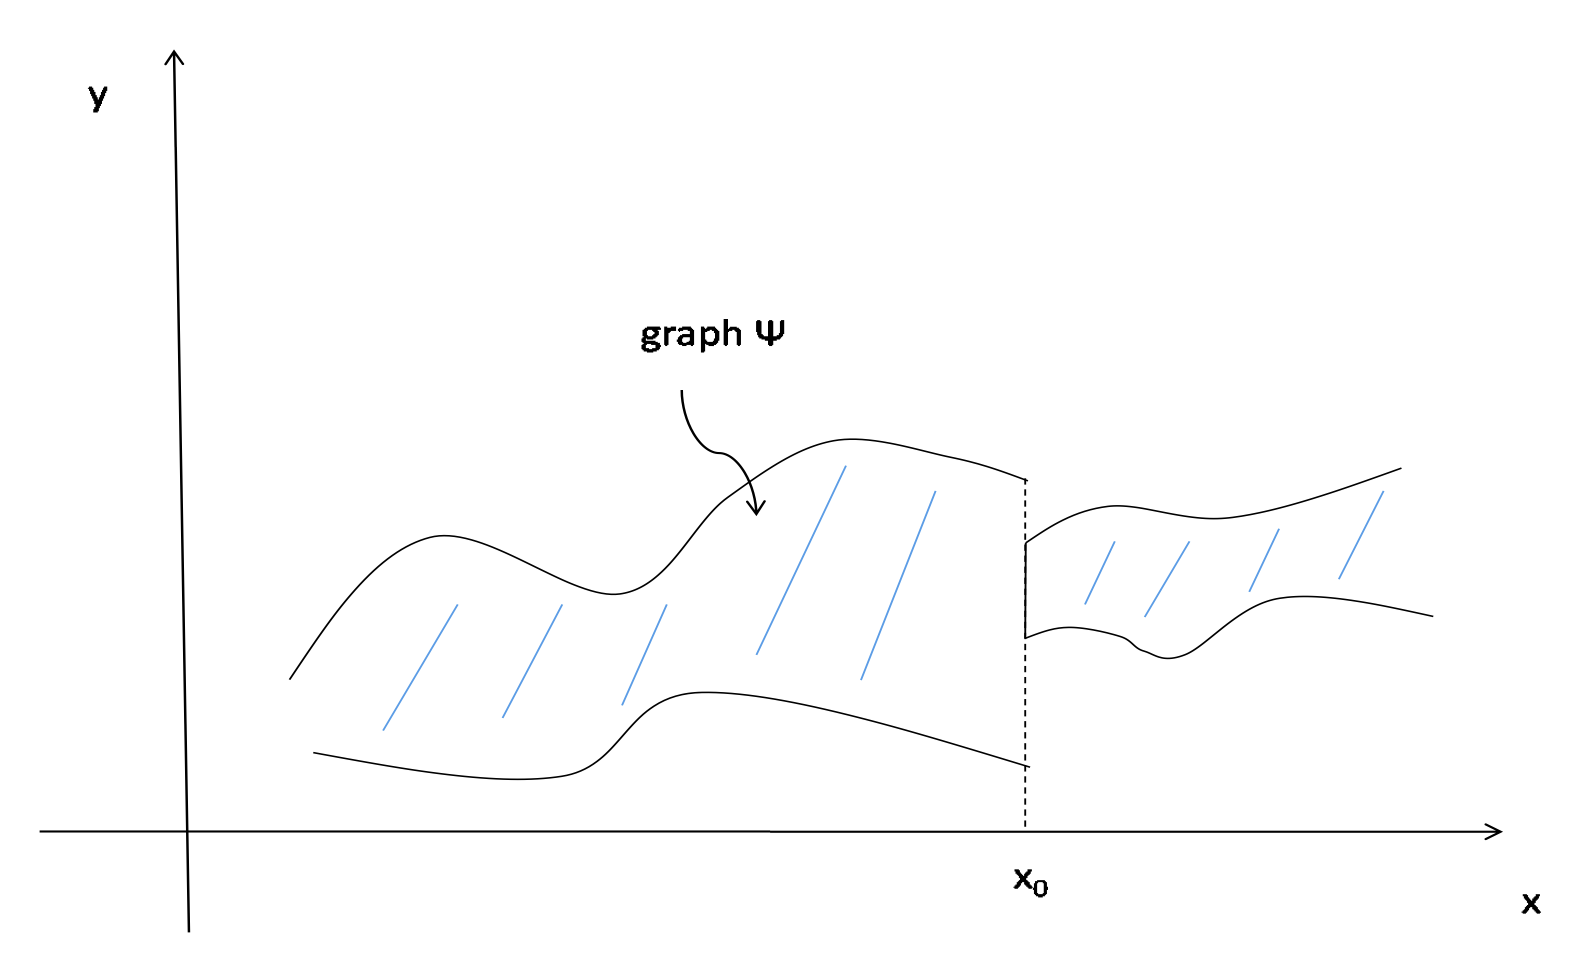
\includegraphics[scale=0.2]{uhc.png}
    \caption{The correspondence $\Psi$ “implodes in the limit” at $x_0$. $\Psi$ is not upper hemicontinuous at $x_0$.}
    \label{}
\end{figure}\end{center}

\begin{center}\begin{figure}[htbp]
    \centering
    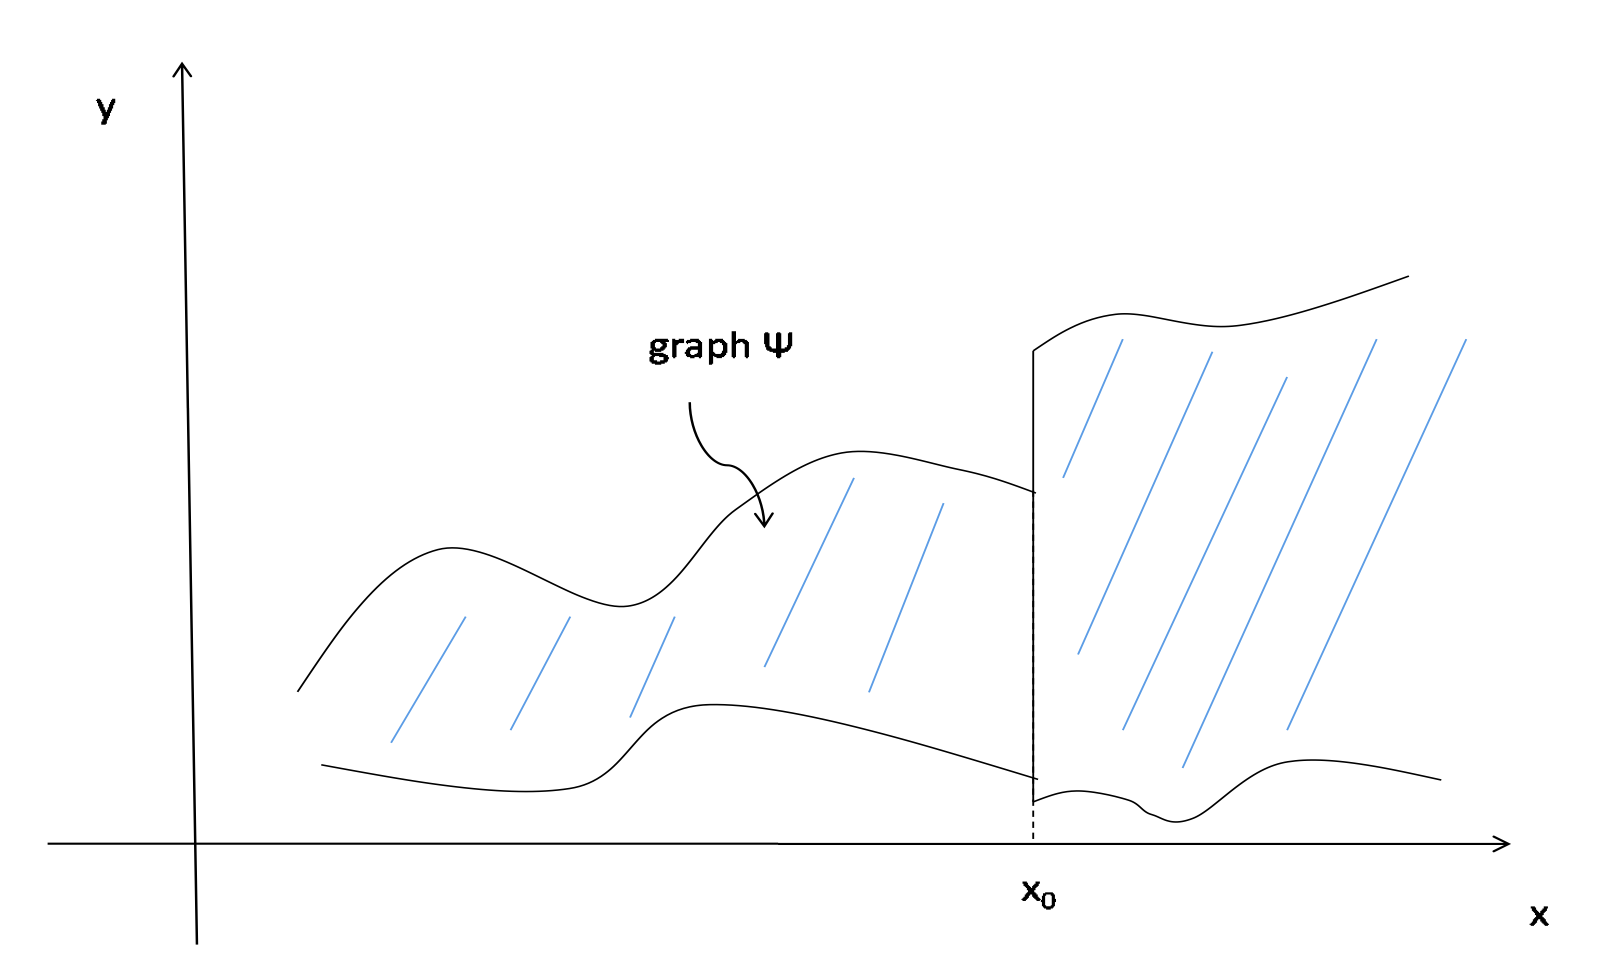
\includegraphics[scale=0.2]{lhc.png}
    \caption{The correspondence $\Psi$ “explodes in the limit” at $x_0$. $\Psi$ is not lower hemicontinuous at $x_0$.}
    \label{}
\end{figure}\end{center}

\subsection{Theorem: $\Psi(x)=\{f(x)\}$ is uhc $\Leftrightarrow$ $f$ is continuous}
\begin{theorem}[$\Psi(x)=\{f(x)\}$ is uhc $\Leftrightarrow$ $f$ is continuous]
    Let $X \subseteq \mathbb{E}^n$, $Y \subseteq \mathbb{E}^m$ and $f : X \rightarrow Y$. Let $\Psi : X \rightarrow  2^Y$ be defined by $\Psi(x) = \{f(x)\}$ for all $x \in X$. Then $\Psi$ is \textbf{uhc} \underline{if and only if} $f$ is \textbf{continuous}.
\end{theorem}


\subsection{Berge's Maximum Theorem: $v(y)=\max_{x\in\Gamma(y)}f(x,y)$ is continuous; $\{x:f(x,y)=v(y)\}$ is uhc with non-empty compact values}
\begin{theorem}[Berge's Maximum Theorem]
    Let $X \subseteq \mathbb{R}^n$ and $Y \subseteq \mathbb{R}^m$. Consider the function $f : X \times Y \rightarrow \mathbb{R}$ and the correspondence $\Gamma : Y \rightarrow 2^X$. Define $v(y) = \max_{x\in\Gamma(y)} f(x, y)$ and $Ω(y) = \argmax_{x\in\Gamma(y)} f(x, y)=\{x:f(x,y)=v(y)\}$. Suppose $f$ and $\Gamma$ are continuous, and that $\Gamma$ has non-empty compact values. Show that v is continuous and $\Omega$ is uhc with non-empty compact values.
\end{theorem}




\section{Graph of Correspondence}
An alternative notion of continuity looks instead at properties of the graph of the correspondence.
\begin{definition}[Graph of Correspondence]
    \normalfont
    The \textbf{graph} of a correspondence $\Psi : X \rightarrow 2^Y$ is the set
    $$\textnormal{graph}\Psi=\{(x,y)\in X\times Y:y\in\Psi(x)\}$$
\end{definition}

\subsection{Closed Graph}
By the definition of continuous function $f:\mathbb{R}^n \rightarrow \mathbb{R}$,  each convergent sequence $\{(x_n, y_n)\}$ in graph $f$ converges to a point $(x, y)$ in graph $f$, that is, graph $f$ is closed.

\begin{definition}[Closed Graph]
    \normalfont
    Let $X\subseteq \mathbb{E}^n$, $Y\subseteq \mathbb{E}^m$. A correspondence $\Psi: X \rightarrow 2^Y$ has closed graph if its graph is a closed subset of $X \times Y$, that is, if for any sequences $\{x_n\} \subseteq X$ and $\{y_n\} \subseteq Y$ such that $x_n \rightarrow x \in X$, $y_n \rightarrow y \in Y$ and $y_n \in \Psi(x_n)$ for each $n$, then $y \in \Psi(x)$.
\end{definition}
\begin{example}
    Consider the correspondence $\Psi(x)=\left\{\begin{matrix}
        \{\frac{1}{x}\},&\textnormal{ if }x\in(0,1]\\
        \{0\},&\textnormal{ if }x=0
    \end{matrix}\right.$ ("implode in the limit")\\
    Let $V = (-0.1, 0.1)$. Then $\Psi(0) = \{0\} \subseteq V$, but no matter how close $x$ is to $0$, $\Psi(x)=\{\frac{1}{x}\}\nsubseteq V$, so $\Psi$ is not uhc at $0$. However, note that $\Psi$ has closed graph.
\end{example}

\section{Closed-valued, Compact-valued, and Convex-valued Correspondences}
\begin{definition}[Closed-valued, Compact-valued, and Convex-valued Correspondences]
    \normalfont
    Given a correspondence $\Psi : X \rightarrow 2^Y$,
    \begin{enumerate}
        \item $\Psi$ is \textbf{closed-valued} if $\Psi(x)$ is a closed subset of $Y$ for all $x$;
        \item $\Psi$ is \textbf{compact-valued} if $\Psi(x)$ is compact for all $x$.
        \item $\Psi$ is \textbf{convex-valued} if $\Psi(x)$ is convex for all $x$.
    \end{enumerate}
\end{definition}

\subsection{Closed-valued, uhc and Closed Graph}
For closed-valued correspondences these concepts can be more tightly connected. A closed-valued and upper hemicontinuous correspondence must have closed graph. For a closed-valued correspondence with a compact range, upper hemicontinuity is equivalent to closed graph.

\begin{theorem}
    Let $X\subseteq \mathbb{E}^n$, $Y\subseteq \mathbb{E}^m$, and $\Psi: X \rightarrow 2^Y$.
    \begin{enumerate}
        \item $\Psi$ is \textbf{closed-valued} and \textbf{uhc} $\Rightarrow$ $\Psi$ has \textbf{closed graph}.
        \item $\Psi$ is \textbf{closed-valued} and \textbf{uhc} $\Leftarrow$ $\Psi$ has \textbf{closed graph}. (If $Y$ is \textbf{compact})
    \end{enumerate}
\end{theorem}

\begin{theorem}
    Let $X\subseteq \mathbb{E}^n$, $Y\subseteq \mathbb{E}^m$, and $\Psi: X \rightarrow 2^Y$. If $\Psi$ has \textbf{closed graph} and there is an \textbf{open set} $W$ with $x_0 \in W$ and a \textbf{compact set} $Z$ such that $x \in W \cap X \Rightarrow \Psi(x) \subseteq Z$, then $\Psi$ is \textbf{uhc} at $x_0$.
\end{theorem}



\subsection{Theorem: compact-valued, uhs correspondence of compact set is compact}
\begin{theorem}\label{thm:compact-valued, uhs correspondence of compact set is compact}
    Let $X$ be a compact set and $\Psi : X \rightarrow 2^X$ be a non-empty, compact-valued upper-hemicontinuous correspondence. If $C \subseteq X$ is compact, then $\Psi(C)$ is compact.
\end{theorem}
\begin{proof}
    Given the compact-valued $\Psi$, we can have an open cover of $\Psi(C)$, $\{U_\lambda:\lambda\in\Lambda\}$. So $\forall x\in C$, there exists $U_{l(x)},l(x)\in\Lambda$ such that $U_{l(x)}$ is an open cover of $\Psi(x)$.

    Consider a $c\in C$. Since $\Psi$ is uhs and $\Psi(c)\subseteq U_{l(c)}$, there exists open set $V_c$ s.t. $c\in V_c$ and $\Psi(x)\subseteq U_{l(c)}, \forall x\in V_c\cap C$.

    $\{V_c:c\in C\}$ is an open cover of $C$. Because $C$ is compact, there is a finite subcover $\{V_{c_i}: i=1,...,m\},m\in \mathbb{N}$, where $\{c_i:i=1,...,m\}\subseteq C$.

    Because $\Psi(x)\subseteq U_{l(c_i)}, \forall x\in V_{c_i}\cap C$ and $\{V_{c_i}: i=1,...,m\},m\in \mathbb{N}$ is a open cover for $C$, we can infer $\{U_{l(c_i)}:i=1,...,m\}$ is a finite subcover of $\{U_{l(c)}:c\in C\}$ for $\Psi(C)$. Hence, $\Psi(C)$ is compact.
\end{proof}

\section{Fixed Points for Correspondences \small{(@ Lec 13 of ECON 204)}}
\subsection{Definition}
\begin{definition}[Fixed Points for Correspondences]
    \normalfont
    Let $X$ be nonempty and $\psi : X \rightarrow 2^X$ be a correspondence. A point $x^* \in X$ is a fixed point of $\psi$ if $x^* \in \psi(x^*)$.
\end{definition}
\begin{note}
    We only need $x^*$ to be in $\psi(x^*)$, not $\{x^*\} = \psi(x^*)$. That is, $\psi$ need not be single-valued at $x^*$. So $x^*$ can be a fixed point of $\psi$ but there may be other elements of $\psi(x^*)$ different from $x^*$.
\end{note}



\subsection{Kakutani's Fixed Point Theorem: uhs, compact, convex values correspondence has a fixed point over compact convex set}
\begin{theorem}[Kakutani's Fixed Point Theorem]
    Let $X \subseteq \mathbb{R}^n$ be a non-empty, \textbf{compact}, \textbf{convex} set and $\psi : X \rightarrow 2^X$ be an \textbf{upper hemi-continuous} correspondence with non-empty, \textbf{compact}, \textbf{convex} values. Then $\psi$ has a fixed point in $X$.
\end{theorem}


\subsection{Theorem: $\exists$ compact set $C = \cap_{i=0}^\infty \Psi^i(X)$ s.t. $\Psi(C)=C$}
\begin{theorem}
    Let $(X, d)$ be a compact metric space and let $\Psi(x) : X \rightarrow 2^X$ be a upper-hemicontinuous, compact-valued correspondence, such that $\Psi(x)$ is non-empty for every $x \in X$. There exists a compact non-empty subset $C\subseteq X$, such that $\Psi(C) \equiv \cup_{x\in C}\Psi(x) = C$.
\end{theorem}
\begin{proof}
    Let's construct a sequence $\{C_n\}$ such that $C_0=X$, $C_1=\Psi(C_0)$, ..., $C_n=\Psi(C_{n-1}),...$ We claim that $C=\cap_{i=0}^\infty C_i$ is a non-empty compact set and satisfies $\Psi(C)=C$.
    \begin{enumerate}
        \item Because we can infer $\Psi(X_1)\subseteq \Psi(X_2)$ if $X_1\subseteq X_2$, $X=C_0\supseteq C_1 \Rightarrow C_1=\Psi(C_0)\supseteq C_2=\Psi(C_1)$,...., so $C_0\supseteq C_1\supseteq \cdots C_n\supseteq \cdots$. Hence, $C$ is not empty.
        \item Because $X$ is compact, by the theorem \ref{thm:compact-valued, uhs correspondence of compact set is compact}, we can infer $C_n$ is compact for all $n$. Then, $C_n$ is closed for all $n$, so $C$ is closed. Because $C$ is a closed set of compact set $X$, $C$ is compact.
        \item $C\subseteq C_n,\forall n \Rightarrow \Psi(C)\subseteq \Psi(C_n),\forall n \Rightarrow \Psi(C)\subseteq C$
        \item Assume $C\subseteq \Psi(C)$ doesn't hold, that is $\exists y\in C$ s.t. $y\notin \Psi(C)$. Because $y\in C$ and $C_0\supseteq C_1\supseteq \cdots C_n\supseteq \cdots$, there exists $k\in C_n$ for all $n$ s.t. $y\in\Psi(k)$. $k\in \cap_{i=1}^\infty C_i=C$, so $\Psi(k)\subseteq \Psi(C)$, which contradicts to $y\notin \Psi(C)$. Hence, $C\subseteq \Psi(C)$.
    \end{enumerate}
    All in all the claim "$C=\cap_{i=0}^\infty C_i$ is a non-empty compact set and satisfies $\Psi(C)=C$" is proved.
\end{proof}


\chapter{Stochastic Dominance}
Based on
\begin{enumerate}[$\circ$]
    \item MIT 14.123 S15 Stochastic Dominance Lecture Notes
    \item Princeton ECO317 Economics of Uncertainty Fall Term 2007 Notes for lectures 4. Stochastic Dominance
\end{enumerate}

\section{First-order Stochastic Dominance}
\subsection{Two Equivalent Definitions}
\begin{definition}[First-order Stochastic Dominance]
    \normalfont
    For any lotteries $F$ and $G$, $F$ \textbf{first-order stochastically dominates} $G$ if and only if the decision maker weakly prefers $F$ to $G$ under every \underline{weakly increasing} utility function $u$, i.e.,
    $$\int u (x) dF \geq \int u(x) dG$$
\end{definition}

\begin{definition}[First-order Stochastic Dominance]
    \normalfont
    For any lotteries $F$ and $G$, $F$ \textbf{first-order stochastically dominates} $G$ if and only if
    $$F(x)\leq G(x),\forall x$$
\end{definition}

\begin{center}\begin{figure}[htbp]
    \centering
    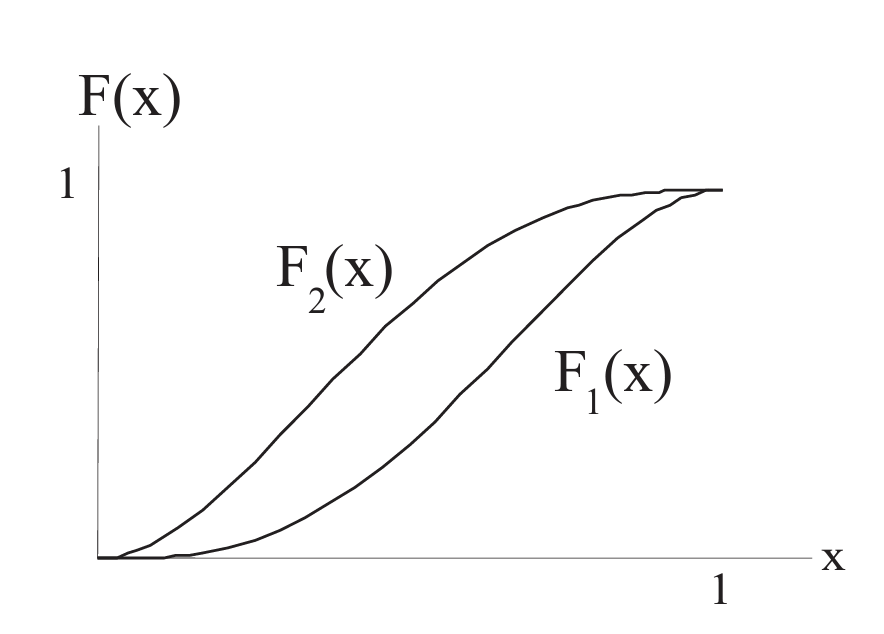
\includegraphics[scale=0.2]{FOSD_1.png}
    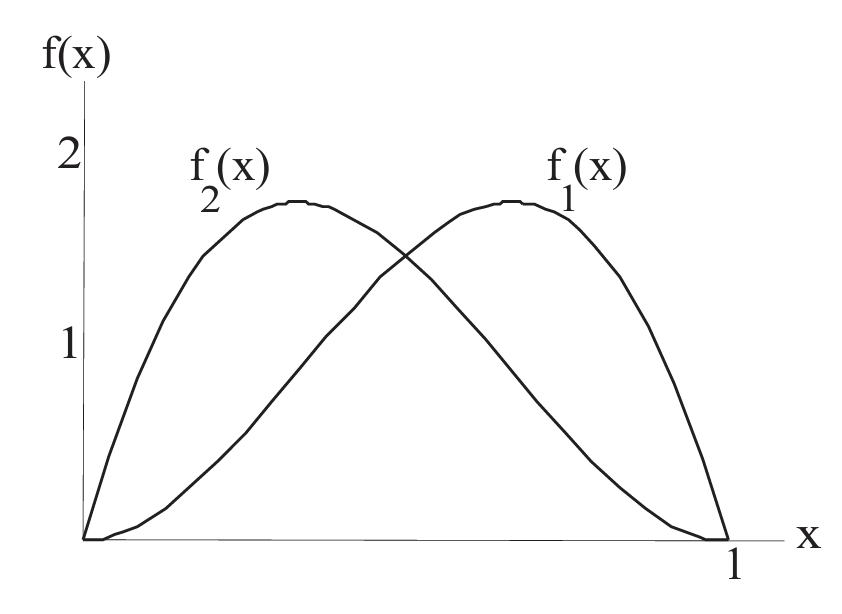
\includegraphics[scale=0.2]{FOSD_2.png}
    \caption{$F_1$ is FOSD over $F_2$: CDF and density comparison}
    \label{}
\end{figure}\end{center}

\section{Second-order Stochastic Dominance}
\subsection{Definition in terms of final goals}
\begin{definition}[Second-order Stochastic Dominance]
    \normalfont
    For any lotteries $F$ and $G$, $F$ \textbf{second-order stochastically dominates} $G$ if and only if the decision maker weakly prefers $F$ to $G$ under every \underline{weakly increasing \textbf{concave}} utility function $u$, i.e.,
    $$\int u (x) dF \geq \int u(x) dG$$
\end{definition}
\begin{center}\begin{figure}[htbp]
    \centering
    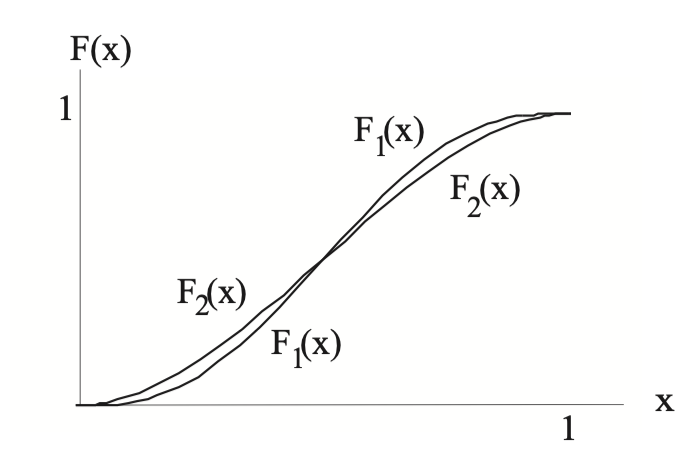
\includegraphics[scale=0.25]{SOSD_1.png}
    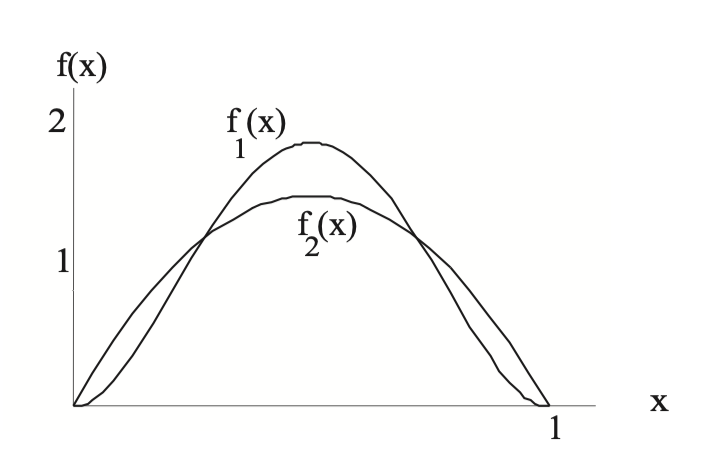
\includegraphics[scale=0.25]{SOSD_2.png}
    \caption{$F_1$ is SOSD over $F_2$: CDF and density comparison}
    \label{}
\end{figure}\end{center}

\subsection{Mean-Preserving Spread}
\begin{definition}[Mean-Preserving Spread]
    \normalfont
    Let $x_F$ and $x_G$ be the random variables associated with lotteries $F$ and $G$. Then $G$ is a \textbf{mean-preserving spread} of $F$ if and only if $$x_G \stackrel{d}{=} x_F+\varepsilon$$
    for some random variable $\varepsilon$ such that $\mathbb{E}(\varepsilon\mid x_F)=0,\forall x_F$.
\end{definition}
The "$\stackrel{d}{=}$" means "is equal in distribution to" (that is, "has the same distribution as").

\begin{note}
    Given $G$ is a \textbf{mean-preserving spread} of $F$, $G$ has larger variance than $F$.
\end{note}

\begin{example}
    $F(198)=\frac{1}{2}, F(202)=\frac{1}{2}$ and $G(100)=\frac{1}{100}$, $G(200)=\frac{98}{100}$, $G(300)=\frac{1}{100}$. Then $$x_G \stackrel{d}{=} x_F+\varepsilon$$
    where the distribution of $\varepsilon$ can be solved by $\left\{\begin{matrix}
        \frac{1}{100}&=\frac{1}{2}P(\varepsilon=102)+\frac{1}{2}P(\varepsilon=98)\\
        \frac{98}{100}&=\frac{1}{2}P(\varepsilon=2)+\frac{1}{2}P(\varepsilon=-2)\\
        \frac{1}{100}&=\frac{1}{2}P(\varepsilon=-98)+\frac{1}{2}P(\varepsilon=-102)
    \end{matrix}\right.$
\end{example}


\subsection{Second-order Stochastic Dominance is equivalent to Mean-Preserving Spread}
\begin{theorem}[Second-order Stochastic Dominance Equivalence]\label{SOSD_equiv}
    Given $\int x dF=\int x dG$ (same mean). The following are equivalent.
    \begin{enumerate}
        \item $F$ second-order stochastically dominates $G$: $\int u (x) dF \geq \int u(x) dG$  for every weakly increasing concave utility function $u$.
        \item $G$ is a mean-preserving spread of $F$.
        \item For every $t\geq 0$, $\int_a^t G(x)dx\geq \int_a^t F(x)dx$.
    \end{enumerate}
\end{theorem}
\begin{center}\begin{figure}[htbp]
    \centering
    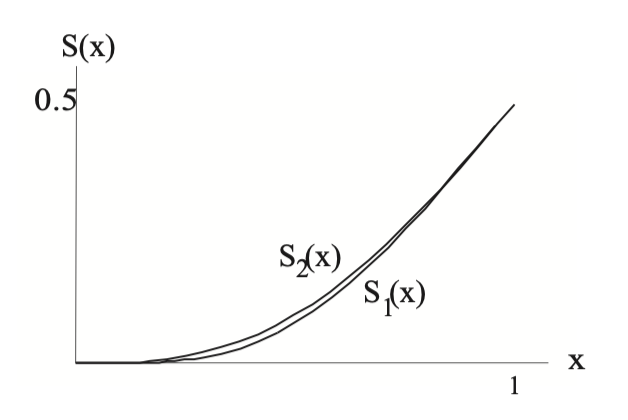
\includegraphics[scale=0.25]{SOSD_3.png}
    \caption{$F_1$ is SOSD over $F_2$, $S(t):\int_a^t F_2(x)dx\geq \int_a^t F_1(x)dx$}
    \label{}
\end{figure}\end{center}


















\chapter{Bayesian Persuasion: Useful Mathematical Results}
Based on
\begin{enumerate}[$\circ$]
    \item Kleiner, A., Moldovanu, B., \& Strack, P. (2021). Extreme points and majorization: Economic applications. \textit{Econometrica}, 89(4), 1557-1593.
    \item 
\end{enumerate}

\section{Majorization}
\subsection{Majorization and Weak Majorization}
\begin{definition}[Majorization]
    \normalfont
    Consider right-continuous functions that map the unit interval $[0,1]$ into the real numbers. For two \underline{non-decreasing} functions $f,g \in L^1$, we say that $f$ \textbf{majorizes} $g$, denoted by $g \prec f$, if the following two conditions hold:
    \begin{equation}
        \begin{aligned}
            \int_x^1 g(s)ds\leq \int_x^1 f(s)ds,\forall x\in [0,1]
        \end{aligned}
        \tag{Condition 1}
        \label{C1}
    \end{equation}
    \begin{equation}
        \begin{aligned}
            \int_0^1 g(s)ds=\int_0^1 f(s)ds
        \end{aligned}
        \tag{Condition 2}
        \label{C2}
    \end{equation}
\end{definition}

\begin{definition}[Weak Majorization]
    \normalfont
    $f$ \textbf{weakly majorizes} $g$, denoted by $g \prec_w f$, if \ref{C1} holds (not necessarily \ref{C2}).
\end{definition}

\subsection{How to work for non-monotonic functions? -- Non-Decreasing Rearrangement}
\begin{note}
    \normalfont
    \textbf{How this work with non-monotonic functions?}\\
    Suppose $f,g$ are non-monotonic, we compare their non-decreasing rearrangements $f^*$, $g^*$.
    \begin{definition}[Rearrangement]
        \normalfont
        Given a function $f$, let $m(x)$ denote the Lebesgue measure of the set $\{s \in[0, 1]: f(s)\leq x\}$, that is $m(x)=\int_{s\in\{s \in[0, 1]: f(s)\leq x\}}1ds$ (the "length" of the set). The non-decreasing rearrangement of $f$, $f^*$, is defined by $$f^*(t) = \inf\{ x \in \mathbb{R}: m(x) \geq t\},\ t\in[0,1]$$
    \end{definition}
\end{note}

\subsection{Generalized Inverse $G^{-1}(x)=\sup\{s:G(s)\leq x\}$}
\begin{definition}[Generalized Inverse]
    \normalfont
    Suppose $G$ is defined on the interval $[0,1]$, we can define the \textbf{generalized inverse}
    $$G^{-1}(x)=\sup\{s:G(s)\leq x\}, x\in [0,1]$$
\end{definition}

\subsection{Theorem: $F$ majorizes $G$ $\Leftrightarrow$ $G$ is a mean-preserving spread of $F$}
Based on
\begin{enumerate}[$\circ$]
    \item Shaked, M., \& Shanthikumar, J. G. (2007). \textit{Stochastic orders}. New York, NY: Springer New York.
\end{enumerate}
Let $X_F$ and $X_G$ be now random variables with distributions $F$ and $G$, defined on the interval $[0,1]$.
\begin{theorem}[Shaked \& Shanthikumar (2007), Section 3.A]
    $$G\prec F \Leftrightarrow F^{-1}\prec G^{-1} \Leftrightarrow X_{G}\leq_{ssd}X_F \textnormal{ and }\mathbb{E}[X_G]=\mathbb{E}[X_F]$$
    where $\leq_{ssd}$ denotes the standard \underline{second-order stochastic dominance}.
\end{theorem}
Based on Theorem \ref{SOSD_equiv}, we can conclude
\begin{corollary}
    \begin{center}
        $F$ majorizes $G$ $\Leftrightarrow$ $G$ is a mean-preserving spread of $F$
    \end{center}
\end{corollary}
That is, we can construct random variables $X_F$, $X_G$,
jointly distributed on some probability space, such that $X_F \sim F$, $X_G \sim G$ and such that $X_F = \mathbb{E}[X_G \mid X_F]$.


\section{Extreme Points}
\subsection{Extreme Points of Convex Set}
\begin{definition}[Extreme Points]
    \normalfont
    An \textbf{extreme point} of a convex set $A$ is a point $x\in A$ that cannot be represented as a convex combination of points in $A$.
\end{definition}

\subsection{Krein-Milman Theorem: Existence of Extreme Points}
\begin{theorem}[Krein-Milman Theorem]\label{KMT}
    Every non-empty \textbf{compact convex} subset of a Hausdorff locally convex topological vector space (for example, a normed space) is the closed, convex hull of its extreme points.\\
    In particular, this set has extreme points.
\end{theorem}


\subsection{Bauer's Maximum Principle: Usefulness of Extreme Points for Optimization}
\begin{theorem}[Bauer's Maximum Principle]\label{BMP}
    Any function that is \textbf{convex and continuous}, and defined on a set that is \textbf{convex and compact}, attains its maximum at some extreme point of that set.
\end{theorem}

\section{Capture Extreme Points in Economic Applications}
Let $L^1$ denote the real-valued and integrable functions defined on $[0,1]$.

We focus on functional maximizers that are non-decreasing, for example, a cumulative distribution function in Bayesian persuasion, or an incentive-compatible allocation in mechanism design.

\begin{definition}
    \normalfont
    \begin{enumerate}
        \item The set of non-decreasing functions that are majorized by $f$ is denoted by $$\textnormal{MPS}(f)=\{g\in L^1\mid g \textnormal{ is non-decreasing and }g\prec f\}$$
        \item The set of non-negative, non-decreasing functions that are weakly majorized by $f$ is denoted by $$\textnormal{MPS}_w(f)=\{g\in L^1\mid g \textnormal{ is non-negative,  non-decreasing and }g\prec f\}$$
        \item The set of non-decreasing functions that majorize $f$ and satisfy $f(0)\leq g\leq f(1)$ is denoted by $$\textnormal{MPC}(f)=\{g\in L^1\mid g \textnormal{ is non-decreasing and }g\succ f \textnormal{ and }f(0)\leq g\leq f(1)\}$$
    \end{enumerate}
\end{definition}

Following two propositions are the Proposition 1 of the Kleiner et al. (2021).
\begin{proposition}[Non-decreasing $f$ $\Rightarrow$ $\textnormal{MPS}(f)$, $\textnormal{MPS}_w(f)$, and $\textnormal{MPC}(f)$ have extreme points]
    Suppose $f\in L^1$ is non-decreasing. Then $\textnormal{MPS}(f)$, $\textnormal{MPS}_w(f)$, and $\textnormal{MPC}(f)$ are convex and compact in the norm topology $\Rightarrow$ (by Krein-Milman Theorem \ref{KMT}) they all have non-empty set of extreme points.
\end{proposition}
\begin{note}
    We use $\textnormal{ext} A$ to denote the set of extreme points of set $A$.
\end{note}
\begin{proposition}[Non-decreasing $f$ $\Rightarrow$ any distribution is a combination of extreme points]
    Suppose $f\in L^1$ is non-decreasing. For any $g\in \textnormal{MPS}(f)$, $\exists$ a probability measure $\lambda_g$ over $\textnormal{ext} \textnormal{MPS}(f)$ such that $$g=\int_{\textnormal{ext} \textnormal{MPS}(f)}h\ d\lambda_g(h)$$
    (also hold for any $g\in \textnormal{MPS}_w(f)$ and $g\in \textnormal{MPC}(f)$).
\end{proposition}

\subsection{Extreme Points in $\textnormal{MPS}(f)$}
\begin{theorem}[Form of Extreme Points in $\textnormal{MPS}(f)$: Kleiner et al. (2021), Theorem 1]
    Let $f$ be non-decreasing. Then $g$ is an \textbf{extreme point} in $\textnormal{MPS}(f)$ \underline{if and only if} there exists a collection of disjoint intervals $\{[\underline{x}_i,\overline{x}_i)\}_{i\in I}$ such that
    \begin{equation}
        \begin{aligned}
            g(x)=\left\{\begin{matrix}
                f(x),&\textnormal{if } x\notin \cup_{i\in I}[\underline{x}_i,\overline{x}_i)\\
                \frac{\int_{\underline{x}_i}^{\overline{x}_i}f(s)ds}{\overline{x}_i-\underline{x}_i},&\textnormal{if } x\in [\underline{x}_i,\overline{x}_i)
            \end{matrix}\right.
        \end{aligned}
        \nonumber
    \end{equation}
\end{theorem}
$g$ is an extreme point of $\textnormal{MPS}(f)$ implies either that $g(x)=f(x)$ or that $g$ is constant at $x$.

\begin{definition}[Exposed Element]
    \normalfont
    An element $x$ of a convex set $A$ is \textbf{exposed} if there exists a continuous linear functional that attains its maximum on $A$ uniquely at $x$.
\end{definition}
\begin{note}
    Every exposed point is extreme, but the converse is not true in general.
\end{note}

\begin{corollary}[Kleiner et al. (2021), Corollary 1]
    Every extreme point of $\textnormal{MPS}(f)$ is exposed.
\end{corollary}

\subsection{Extreme Points in $\textnormal{MPS}_w(f)$}
For a set $A\subseteq [0,1]$, we use $\mathbf{1}_{A}(x)$ denote the indicator function of set $A$: it equals to $1$ if $x\in A$ and $0$ otherwise.
\begin{corollary}
    Suppose that $f$ is non-decreasing and non-negative. A function $g$ is an extreme point of $\textnormal{MPS}_w(f)$ \underline{if and only if} there is $\theta \in[0,1]$ such that $g$ is an extreme point of $\textnormal{MPS}(f)$ and $g(x) = 0$ for $x\in[0,\theta)$.
\end{corollary}









\end{document}